This subsection is used when we have to save or retrive data from the database. When user tries to login, register, add self, add item or search we have to use database. When somebody wants to register for the app, he provides all the infomration then these information is taken by the DB controller and saved in organized manner. same process occurs for all the other activities like adding self, adding item or login.
\subsection{DB Controller}
This is a type of main controller of the Database system. All the data that needs to be stored in database is first handled by this layer and later stored in the database. When any of the other layer send data to the database layer, first database layer takes the information and figures out what type of data is provided and what to do with the given data.

\begin{figure}[h!]
	\centering
 	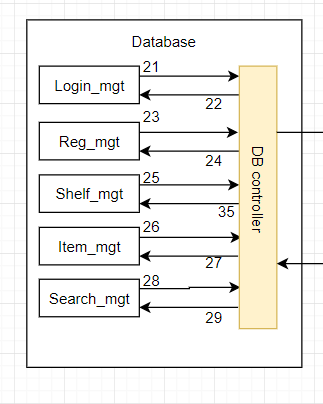
\includegraphics[width=0.60\textwidth]{images/dbcontroller}
 \caption{DB Controller description diagram}
\end{figure}

\subsubsection{Assumptions}
These are the following assumptions made about this subsection:
\begin{itemize}
    \item All the input provided to be saved in the database is a valid input.
    \item Device is connected to the internet when saving or retrieving the data.
\end{itemize}

\subsubsection{Responsibilities}
These are the following responsibilities of the Database Controller.
\begin{itemize}
    \item It must be able to take input sent from all the other layers.  
    \item When input is captured it must be able to classify if the data is login data or sign up data. Must be able to classify if the incoming data is trying to search the item or save the item in the database.
\end{itemize}

\subsubsection{Subsystem Interfaces}


\begin {table}[H]
\caption {Subsystem interfaces} 
\begin{center}
    \begin{tabular}{ | p{1cm} | p{6cm} | p{3cm} | p{3cm} |}
    \hline
    ID & Description & Inputs & Outputs \\ \hline
    \#22 & DB controller/Login\_mgt & \pbox{3cm}{N/A } & \pbox{3cm}{Username\\ Password}  \\ \hline
    \#21 & Login\_mgt/DB Controller & \pbox{3cm}{Success Message \\ Failure Message} & \pbox{3cm}{N/A}  \\ \hline
    
    \#24 & DB Controllere/Reg\_mgt & \pbox{3cm}{N/A} & \pbox{3cm}{Username\\ Password\\email address\\User Name}  \\ \hline
    \#23 & Reg\_mgt/DB Controller & \pbox{3cm}{Success Message \\ Failure Message1} & \pbox{3cm}{N/A}  \\ \hline
    
    \#35 & DB Controller/Shelf\_mgt & \pbox{3cm}{N/A} & \pbox{3cm}{Shelf Name\\Row\\column\\Shelf Location}  \\ \hline
    \#25 & Shelf\_mgt/DB Controller & \pbox{3cm}{Success Message \\ Failure Message} & \pbox{3cm}{N/A}  \\ \hline
    
     \#26 & DB Controller/Item\_mgt & \pbox{3cm}{N/A} & \pbox{3cm}{Item name \\ BarCode(opt) \\ Quantity\\ Expiration Date(opt)\\ Expiration\_notification(opt)\\ PIN(opt)\\Brewery(if alcohol)\\ Style(if alcohol)}  \\ \hline
     \#27 & DB Controller/Item\_mgt & \pbox{3cm}{Image file} & \pbox{3cm}{N/A}  \\ \hline
    
     \#28 & DB Controller/Search\_mgt & \pbox{3cm}{N/A} & \pbox{3cm}{User input \\ label}  \\ \hline
    \#29 & Search\_mgt/DB Controller & \pbox{3cm}{Success Message \\ Failure Message \\ Item image} & \pbox{3cm}{N/A}  \\ \hline
    \end{tabular}
\end{center}
\end{table}

\subsection{Login Mgt}
This subsection of database just deals with the login information. User first registers for the account in the mobile application. Then when he wants to use the app he will provide the user name and password for the app. Then the login management layer handles all the data. It checks if the user name and password provided by the user exists in database or not. It should allow user to login if the combination of user name and password exists else it should deny user from using the application itself.

\begin{figure}[h!]
	\centering
 	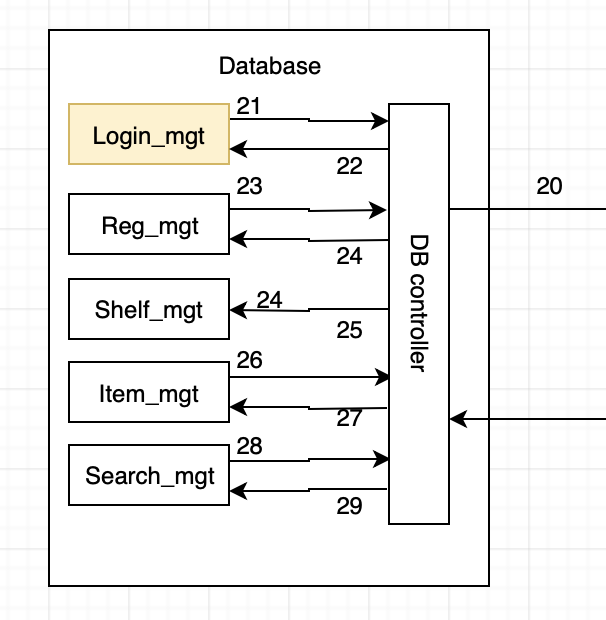
\includegraphics[width=0.60\textwidth]{images/loginmgt}
 \caption{Login mgt description diagram}
\end{figure}

\subsubsection{Assumptions}
These are the following assumptions made about this subsection:
\begin{itemize}
    \item Input provided by the user is valid input. Inputs are not malicious code or SQL query.
\end{itemize}

\subsubsection{Responsibilities}
These are the following responsibilities of this layer;
\begin{itemize}
    \item Check the provided login against the database login information.
    \item If provided login data exists in database let user log in to the app else reject from logging in.
\end{itemize}

\subsubsection{Subsystem Interfaces}
Each of the inputs and outputs for the subsystem are defined here. Create a table with an entry for each labelled interface that connects to this subsystem. For each entry, describe any incoming and outgoing data elements will pass through this interface.

\begin {table}[H]
\caption {Subsystem interfaces} 
\begin{center}
    \begin{tabular}{ | p{1cm} | p{6cm} | p{3cm} | p{3cm} |}
    \hline
    ID & Description & Inputs & Outputs \\ \hline
    \#22 & DB controller/Login\_mgt & \pbox{3cm}{N/A } & \pbox{3cm}{Username\\ Password}  \\ \hline
    \#21 & Login\_mgt/DB Controller & \pbox{3cm}{Success Message \\ Failure Message} & \pbox{3cm}{N/A}  \\ \hline
    \end{tabular}
\end{center}
\end{table}

\subsection{Register Mgt}
This subsection of the database deals with registration data like first name, last name, DOB,etc. When user provides the information it is validated for SQL injection and passed into the register management. Then the data is stored in database in organized manner by the register management subsystem.

\begin{figure}[h!]
	\centering
 	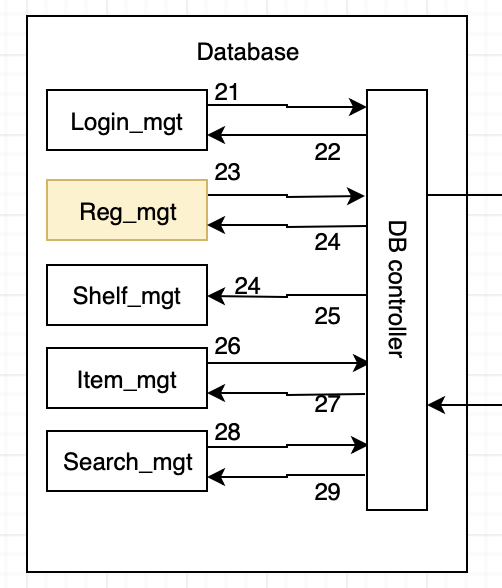
\includegraphics[width=0.60\textwidth]{images/regmgt}
 \caption{Register mgt description diagram}
\end{figure}

\subsubsection{Assumptions}
These are the following assumptions made about this subsection:
\begin{itemize}
    \item User provides all the information needed to register the application. 
    \item Input provided by user is already verified to be the valid input. Eg, malicious code or SQL query is already discarded.
\end{itemize}

\subsubsection{Responsibilities}
These are the following responsibilities of this subsection.
\begin{itemize}
    \item Must be able to return error if all of input field is not provided.
    \item Must be able to store all the information in the database in easy retrieval fashion.
\end{itemize}

\subsubsection{Subsystem Interfaces}
Each of the inputs and outputs for the subsystem are defined here. Create a table with an entry for each labelled interface that connects to this subsystem. For each entry, describe any incoming and outgoing data elements will pass through this interface.

\begin {table}[H]
\caption {Subsystem interfaces} 
\begin{center}
    \begin{tabular}{ | p{1cm} | p{6cm} | p{3cm} | p{3cm} |}
    \hline
    ID & Description & Inputs & Outputs \\ \hline
    \#24 & DB Controllere/Reg\_mgt & \pbox{3cm}{N/A} & \pbox{3cm}{Username\\ Password\\email address\\User Name}  \\ \hline
    \#23 & Reg\_mgt/DB Controller & \pbox{3cm}{Success Message \\ Failure Message1} & \pbox{3cm}{N/A}  \\ \hline
    \end{tabular}
\end{center}
\end{table}

\subsection{Shelf mgt}
This subsystem of database is used whenever user wants to add or remove self. When user provides the specification for the self then the database controller takes the data and passes it to the self management layer. Then the layer takes the information and makes the necessary adjustment in the database.
\begin{figure}[h!]
	\centering
 	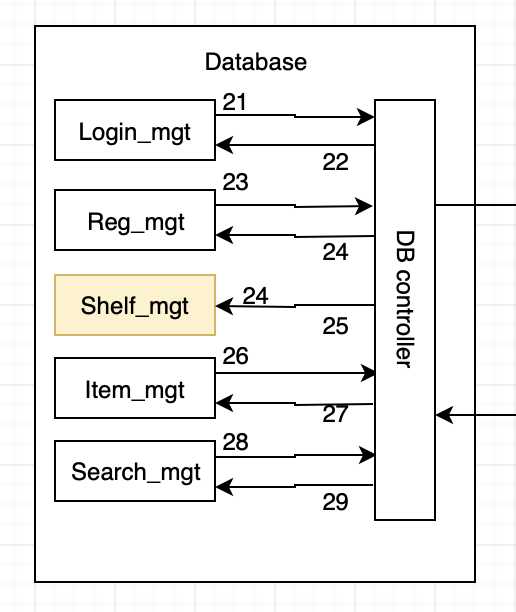
\includegraphics[width=0.60\textwidth]{images/shelfmgt}
 \caption{Shelf mgt description diagram}
\end{figure}

\subsubsection{Assumptions}
These are the following assumptions made about this subsection:
\begin{itemize}
    \item Input provided by user is already verified to be the valid input. Eg, malicious code or SQL query's already discarded.
    \item All the necessary input for adding or deleting the self is provided.
\end{itemize}

\subsubsection{Responsibilities}
These are the following responsibility's that must be performed by this sub system:
\begin{itemize}
    \item Must be able to take all the input values and allocate or de-allocate the self space according to the input values.
\end{itemize}

\subsubsection{Subsystem Interfaces}
Each of the inputs and outputs for the subsystem are defined here. Create a table with an entry for each labelled interface that connects to this subsystem. For each entry, describe any incoming and outgoing data elements will pass through this interface.

\begin {table}[H]
\caption {Subsystem interfaces} 
\begin{center}
    \begin{tabular}{ | p{1cm} | p{6cm} | p{3cm} | p{3cm} |}
    \hline
    ID & Description & Inputs & Outputs \\ \hline
      \#35 & DB Controller/Shelf\_mgt & \pbox{3cm}{N/A} & \pbox{3cm}{Shelf Name\\Row\\column\\Shelf Location}  \\ \hline
    \#25 & Shelf\_mgt/DB Controller & \pbox{3cm}{Success Message \\ Failure Message} & \pbox{3cm}{N/A}  \\ \hline
    \end{tabular}
\end{center}
\end{table}

\subsection{Item mgt}
This subsystem of the database is used whenever user wants to add or remove item from the database. When user provides the data for adding or removing the item, then the DB controller takes the input at first and then passes it to the item Mgmt. Then the layer takes the input value and make necessary change ie. add or remove the item accordingly.

\begin{figure}[h!]
	\centering
 	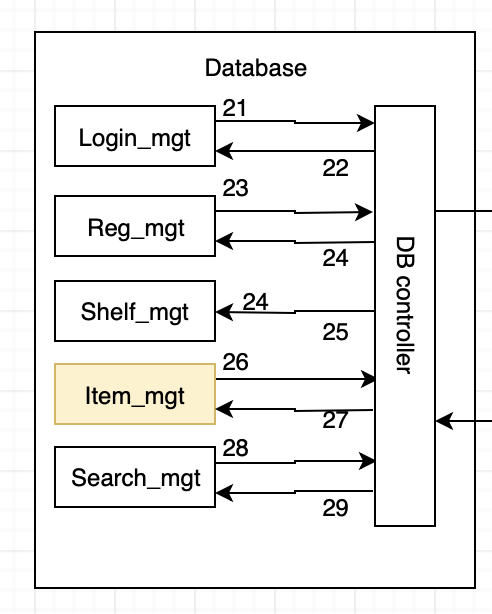
\includegraphics[width=0.60\textwidth]{images/itemmgt}
 \caption{Item mgt description diagram}
\end{figure}

\subsubsection{Assumptions}
These are the following assumptions made about this subsection:
\begin{itemize}
    \item Input provided by user is already verified to be the valid input. Eg, malicious code or SQL query is already discarded.
    \item All the input value is provided by the user.
\end{itemize}

\subsubsection{Responsibilities}
These are the following responsibilities of this subsystem.
\begin{itemize}
    \item Must be able to take all the input values and add or remove item according to the input provided by the user.
\end{itemize}

\subsubsection{Subsystem Interfaces}
Each of the inputs and outputs for the subsystem are defined here. Create a table with an entry for each labelled interface that connects to this subsystem. For each entry, describe any incoming and outgoing data elements will pass through this interface.

\begin {table}[H]
\caption {Subsystem interfaces} 
\begin{center}
    \begin{tabular}{ | p{1cm} | p{6cm} | p{3cm} | p{3cm} |}
    \hline
    ID & Description & Inputs & Outputs \\ \hline
    \#26 & DB Controller/Item\_mgt & \pbox{3cm}{N/A} & \pbox{3cm}{Item name \\ BarCode(opt) \\ Quantity\\ Expiration Date(opt)\\ Expiration\_notification(opt)\\ PIN(opt)\\Brewery(if alcohol)\\ Style(if alcohol)}  \\ \hline
     \#27 & DB Controller/Item\_mgt & \pbox{3cm}{Success Message \\ Failure Message} & \pbox{3cm}{N/A}  \\ \hline
    \end{tabular}
\end{center}
\end{table}

\subsection{Search mgt}
This Sub System deals with taking the item description from user and it searches for the item. Variety of options are provided for searching the item. User can use the camera in the cellphone to scan the QR generated for the specific item or users will also be able to search the item by their names.

\begin{figure}[h!]
	\centering
 	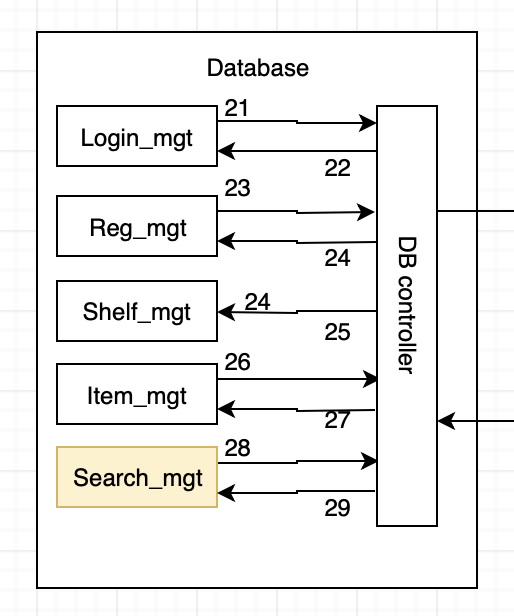
\includegraphics[width=0.60\textwidth]{images/searchmgt}
 \caption{Search mgt description diagram}
\end{figure}

\subsubsection{Assumptions}
These are the following assumptions made about this subsection:
\begin{itemize}
    \item Input provided by user is already verified to be the valid input. Eg, malicious code or SQL query is already discarded.
    \item All the necessary information is provided for the search. 
    \item Device has working camera to scan and search. 
\end{itemize}

\subsubsection{Responsibilities}
These are the following responsibilities of this sub system:
\begin{itemize}
    \item Must be able to take the input and return the result if it exists in database and return "No Items Found" if nothing is found in the database.
\end{itemize}

\subsubsection{Subsystem Interfaces}
Each of the inputs and outputs for the subsystem are defined here. Create a table with an entry for each labelled interface that connects to this subsystem. For each entry, describe any incoming and outgoing data elements will pass through this interface.

\begin {table}[H]
\caption {Subsystem interfaces} 
\begin{center}
    \begin{tabular}{ | p{1cm} | p{6cm} | p{3cm} | p{3cm} |}
    \hline
    ID & Description & Inputs & Outputs \\ \hline
    \#28 & DB Controller/Search\_mgt & \pbox{3cm}{N/A} & \pbox{3cm}{User input \\ label}  \\ \hline
    \#29 & Search\_mgt/DB Controller & \pbox{3cm}{Success Message \\ Failure Message \\ Item image} & \pbox{3cm}{N/A}  \\ \hline
    \end{tabular}
\end{center}
\end{table}
